\documentclass[10pt]{article}
\usepackage[english]{babel}
\usepackage[latin1]{inputenc}
\usepackage{subfigure}
\usepackage{epsfig}
\usepackage{amsmath}
\parindent 0mm
\textwidth 16cm
\textheight 23cm
\oddsidemargin 0cm
\evensidemargin 0cm
\topmargin -10mm
\begin{document}
\pagestyle{empty}
\begin{Large}
\begin{bf} 
T-61.5130 Machine Learning and Neural Networks\\ 
\end{bf}
\end{Large}
Karhunen, Tele Hao\\  
\\
\begin{large}
\begin{bf}
Exercise 1,  4.11.2011
\end{bf}
\end{large}
\begin{enumerate}

\item An odd sigmoid function is defined by
\begin{equation*}
\varphi(v)=\frac{1-\exp(-av)}{1+\exp(-av)}=\tanh(av/2),
\end{equation*}
where $\tanh$ denotes a hyperbolic tangent. The limiting values of
this second sigmoid function are $-1$ and $+1$. Show that the derivate 
of $\varphi(v)$ with respect to $v$ is given by
\begin{equation*}
\frac{d\varphi}{dv}=\frac{a}{2}(1-\varphi^2(v)).
\end{equation*}
What is the value of this derivate at the origin? Suppose that the
slope parameter $a$ is made infinitely large. What is the resulting
form of $\varphi(v)$?

\item 
\begin{enumerate} \item Show that the McCulloch-Pitts formal model of
a neuron may be approximated by a sigmoidal neuron (i.e., neuron using 
a sigmoid activation function with large synaptic weights). 
\item Show that a linear neuron may be approximated by a sigmoidal
neuron with small synaptic weights. 
\end{enumerate}

\item Construct a fully recurrent network with 5 neurons, but with no
self-feedback. 


\item Consider a multilayer feedforward network, all the neurons of
which operate in their linear regions. Justify the statement that such 
a network is equivalent to a single-layer feedforward network. 

\item 
\begin{enumerate} \item Figure 1(a) shows the
signal-flow graph of a recurrent network made up of two neurons. Write
the nonlinear difference equation that defines the evolution of $x_1(n)$
or that of $x_2(n)$. These two variables define the outputs of the top 
and bottom neurons, respectively. What is the order of this equation? 
\item Figure 1(b) shows the signal-flow graph of a recurrent network
consisting of two neurons with self-feedback. Write the coupled system 
of two first-order nonlinear difference equations that describe the
operation of the system.
\end{enumerate}
\end{enumerate}

\begin{figure}[h] 
\centering
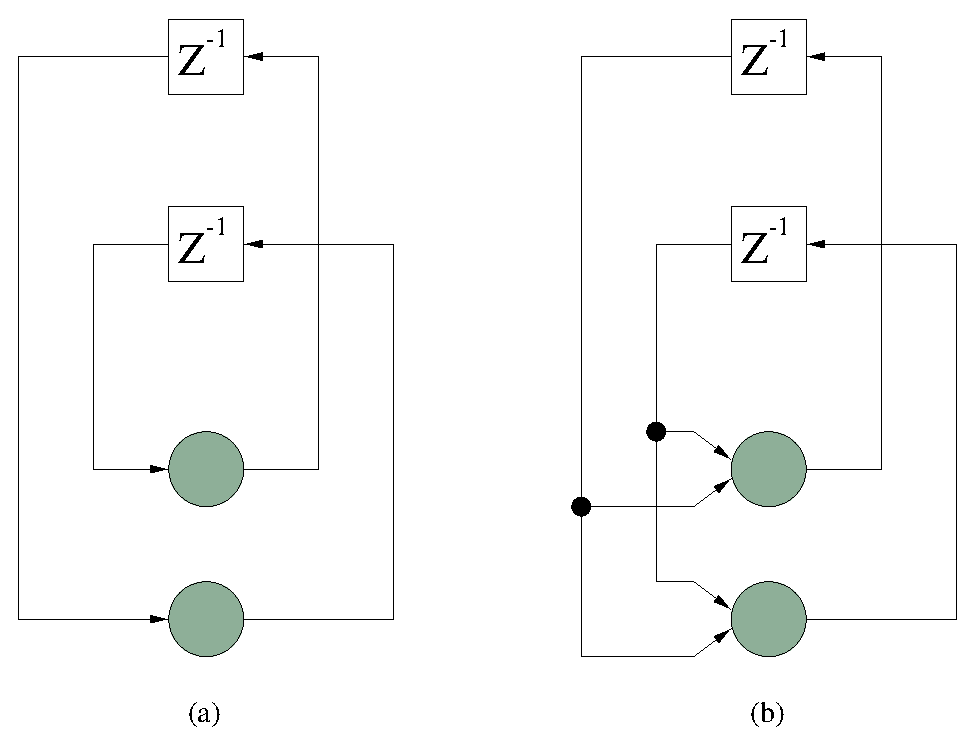
\epsfig{file=neuroEx1_4ab.eps,width=80mm}
\caption{The signal-flow graphs of the two recurrent networks.}
\label{fig:ex4ab}
\end{figure}


\end{document}             % End of document.
